% Created 2017-04-10 Mon 08:00
\documentclass[11pt]{article}
\usepackage[utf8]{inputenc}
\usepackage[T1]{fontenc}
\usepackage{fixltx2e}
\usepackage{graphicx}
\usepackage{longtable}
\usepackage{float}
\usepackage{wrapfig}
\usepackage{rotating}
\usepackage[normalem]{ulem}
\usepackage{amsmath}
\usepackage{textcomp}
\usepackage{marvosym}
\usepackage{wasysym}
\usepackage{amssymb}
\usepackage{hyperref}
\tolerance=1000
\date{April 10, 2017}
\title{Week 12 lecture notes - PSYC 3435}
\hypersetup{
  pdfkeywords={},
  pdfsubject={},
  pdfcreator={Emacs 25.1.1 (Org mode 8.2.10)}}
\begin{document}

\maketitle
This is a short week due to Easter\ldots{} we will talk about quasi-experimental designs

\section*{Definitions}
\label{sec-1}

A \emph{quasi-experiment} is a type of research design where a comparison is made, but \textbf{no random assignment} occurs

Examples:
\begin{itemize}
\item studies with \emph{subject variables} (e.g., high vs. low IQ, males vs. females, smokers vs. nonsmokers, etc.)
\item time is used as a variable (e.g., pretest-posttest, developmental designs [more on this later])
\end{itemize}

\section*{Pretest-posttest designs}
\label{sec-2}

In a pretest/posttest design, a behavior is measured \emph{twice}
\begin{itemize}
\item once before treatment (pretest)
\item once after treatment (posttest)
\end{itemize}

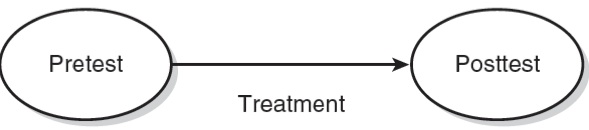
\includegraphics[width=.9\linewidth]{figures/prePost.jpg}

But\ldots{}
\begin{itemize}
\item \emph{history effects} -- events that occur during the course of a study that can result in bias
\item \emph{maturation} -- natural changes that happen to participant during course of study
\end{itemize}

Better: pretest/posttest with \emph{nonequivalent groups}

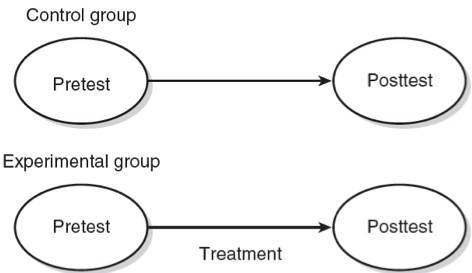
\includegraphics[width=.9\linewidth]{figures/prePost2.jpg}

But..
\begin{itemize}
\item \emph{testing effects} - occur when participants are tested multiple times and each subsequent test is affected by the previous tests
\end{itemize}

Even better: Solomon four-group design

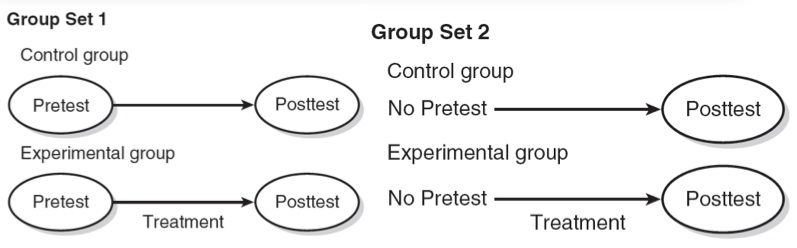
\includegraphics[width=.9\linewidth]{figures/solomon.jpg}

Method: compare posttest scores across group sets
\begin{itemize}
\item if no differences between Group Set 1 and Group Set 2, then no testing effects have occurred.
\end{itemize}
% Emacs 25.1.1 (Org mode 8.2.10)
\end{document}